\documentclass{standalone}
\usepackage{tikz}
\usepackage{ctex,siunitx}
\setCJKmainfont{Noto Serif CJK SC}
\usepackage{tkz-euclide}
\usepackage{amsmath}
\usetikzlibrary{patterns, calc}
\usetikzlibrary {decorations.pathmorphing, decorations.pathreplacing, decorations.shapes,}

\begin{document}
\small
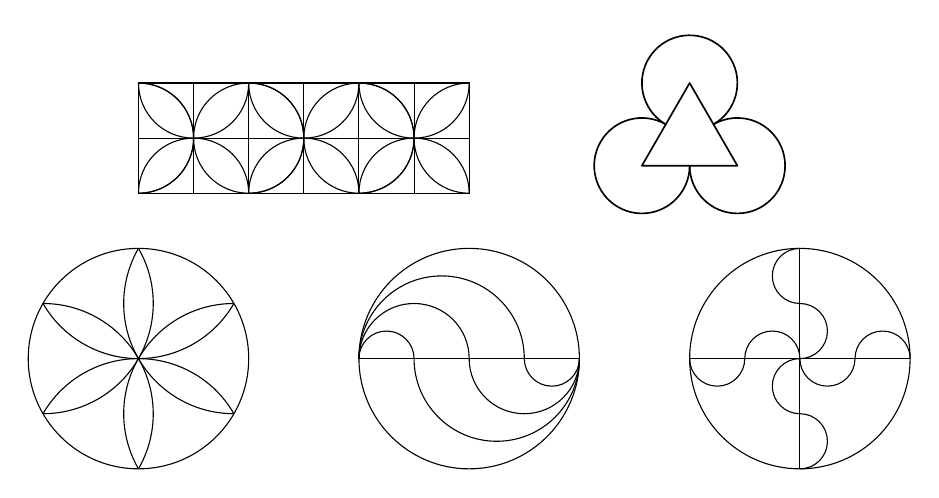
\begin{tikzpicture}[>=stealth,scale=0.7]
  \tkzSetUpPoint[fill=black]
  % \useasboundingbox(-1,-0.75)rectangle(3.7,1.4);
  \begin{scope}
  \draw(0,0) rectangle (2,2);
  \draw(2,0) rectangle (4,2);
  \draw(4,0) rectangle (6,2);
  \foreach \x in {0,2,4}
  {
  \draw(\x+1,0)--(\x+1,2);
  \draw(\x,0) arc (-90:90:1);
  \draw(\x,0) arc (180:0:1);
  \draw(\x,2) arc (90:-90:1);
  \draw(\x,2) arc (180:360:1);
  	\draw(\x+2,0) arc (270:90:1);
  }
  \draw(0,1)--(6,1);
  \end{scope}
  \begin{scope}[xshift=10cm,yshift=1cm]
  \tkzDefPoint(90:1){A}
  \tkzDefPoint(210:1){B}
  \tkzDefPoint(-30:1){C}
  \tkzDefMidPoint(A,B)\tkzGetPoint{F}
  \tkzDefMidPoint(A,C)\tkzGetPoint{E}
  \tkzDefMidPoint(B,C)\tkzGetPoint{D}
  \tkzDrawArc[semithick](A,E)(F)
  \tkzDrawArc[semithick](B,F)(D)
  \tkzDrawArc[semithick](C,D)(E)
  \tkzDrawPolygon[semithick](A,B,C)
  \end{scope}
  \begin{scope}[yshift=-3cm]
  \draw(0,0)circle(2);
  \draw(30:2) arc (90:210:2);
  \draw(30:2) arc (-30:-150:2);
  \draw(-30:2) arc (-90:-210:2);
  \draw(-30:2) arc (30:150:2);
  \draw(90:2) arc (30:-90:2);
  \draw(-90:2) arc (-30:90:2);
  \end{scope}
  \begin{scope}[xshift=4cm, yshift=-3cm]
  \draw(2,0)circle(2);
  \foreach \x in {1,2,3}
  {
  \draw(0,0) arc (180:0:\x/2);
  \draw(4,0) arc (0:-180:\x/2);
  }
  \draw(0,0)--(4,0);
  \end{scope}
  \begin{scope}[xshift=12cm, yshift=-3cm]
  \draw(0,0)circle(2);
  \draw(-2,0)--(2,0);
  \draw(0,-2)--(0,2);
  \foreach \x in {0,2}
  {
  \draw(\x-2,0) arc (-180:0:.5);
  \draw(\x-1,0) arc (180:0:.5);
  \draw(0,\x) arc (90:270:.5);
  \draw(0,\x-1) arc (90:-90:.5);
  }
  \end{scope}
\end{tikzpicture}
\end{document}